 \subsection{Barcode} \label{barcode}
Om de verschillende schermen te identificeren wordt gebruik gemaakt van een kleuren barcode. De barcode bestaat uit een herhalend patroon van 5 unieke kleuren telkens gevolgd door een witte lijn. Door het gebruik van deze witte lijn weet het algoritme waar het patroon eindigt en de volgende sequentie terug opnieuw begint. Het detecteren van deze 5 kleuren gebeurt aan de hand van opgestelde HSL ranges, zie \ref{Ranges}. Voor de identificatie van de slaves wordt dus een unieke combinatie van deze 5 kleuren weergegeven, zie figuur \ref{scherm}. Deze vormt dan een unieke vijfcijferige code, die gelinkt kan worden aan de bijhorende slave. Dit zorgt ervoor dat we in theorie een totaal van $5!$ ($=120$) verschillende schermen op één moment kunnen detecteren. Herhaling van het patroon heeft als resultaat dat bij overlap het scherm nog steeds geïdentificeerd kan worden. Het algoritme zal twee keer over alle pixels itereren. Hierdoor heeft het algorimte een tijdscomplexiteit van
\[O(2mn)=O(mn)\]
met m en n de dimensies van het eiland waarin de barcode gelezen wordt. Het algoritme gaat een keer horizontaal en een keer verticaal over de pixels. Op deze manier kan de barcode in alle mogelijke orientaties van het scherm gelezen worden. Vervolgens worden de HSL waarden van deze pixels bekeken om de overeenkomstige kleur van elke pixel te achterhalen. Wanneer een HSL waarde binnen de gewenste range valt, wordt het overeenkomstig cijfer opgeslaan in een lijst. Bij het bereiken van een witte lijn weet het algoritme dat het aan het einde van het patroon is. Wanneer dit het geval is, wordt het inlezen van de volledige vijfcijferige code gecontroleerd op volledigheid. Zo niet, wordt de lijst leeg gehaald en zoekt het algoritme verder. Het herhalend patroon is dus essentieel aan het correct inlezen van de barcode. Een groter aantal herhalingen stemt overeen met een hogere kans op mogelijke detectie, maar stemt ook overeen met een kleinere oppervlakte per herhaling. Deze kleinere oppervlakte is dan weer nadelig voor detectie. Aangezien hiermee de kans stijgt dat een kleur niet gededecteerd wordt. Nadat het algoritme over alle pixels geweest is, wordt de ratio berekend tussen de code die het meeste keer gelezen is en de totale aantal codes die zijn gelezen. Deze ratio bepaalt dan of de code, die door de horizontale iteratie of door de verticale iteratie het meest gelezen is, gebruikt wordt.

\begin{figure}[h!]
	\center
	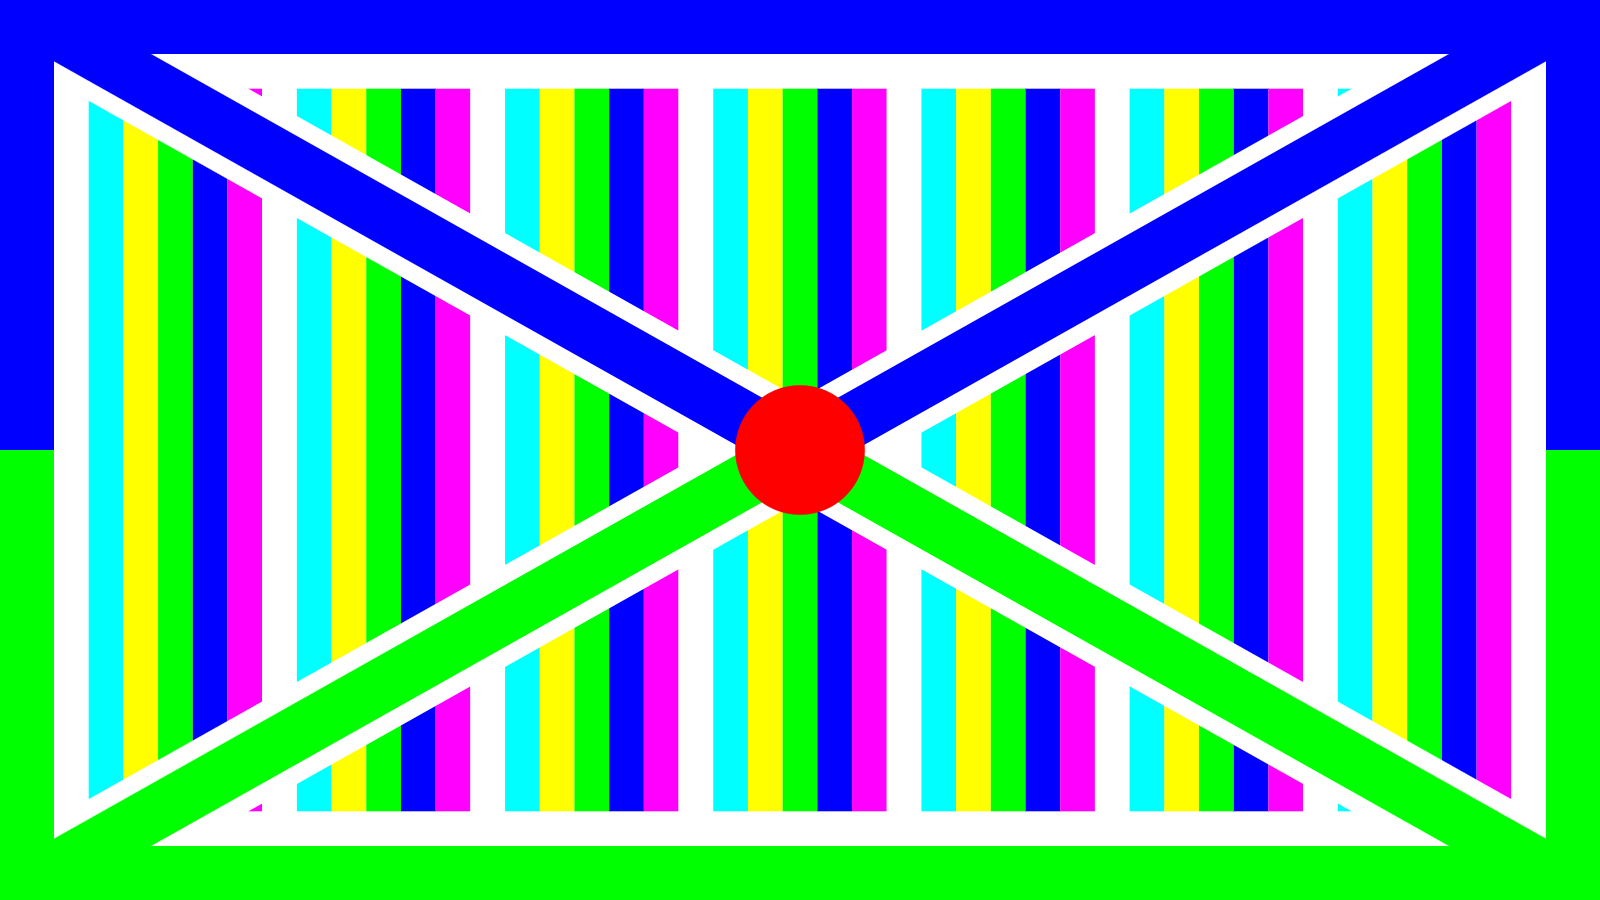
\includegraphics[width=0.8\textwidth]{img/screen.png}
	\caption{Scherm met randen en kruis voor detectie met barocde erachter voor identificatie.}
	\label{scherm}
\end{figure}

\subsection{Verdere verbeteringen}
Zoals reeds vermeld in \ref{Verbeteringen kleur} is het individueel dedecteren van zoveel verschillende kleuren geen goed idee. Dit is dan ook de reden dat andere opties reeds bekeken worden. Zoals ook reeds vermeld zou een eerste optie zijn om te kijken naar het contrast tussen de opeenvolgende kleuren in plaats van de kleuren apart te dedecteren. Een andere optie die bekeken wordt is het overschakelen naar een zwart-wit barcode waarbij gebruik gemaakt wordt van het contrast tussen zwart en wit. Een andere mogelijke verbetering is het aantal herhalingen afhankelijk maken van de grootte van het scherm. Dit heeft als voordeel dat het aantal herhalingen geoptimaliseerd is voor de grootte van het scherm.
